\subsection{Связь магнитных и электрических полей}

Запишем закон Био-Савара-Лапласа для электрона:

\setlength\intextsep{0.5cm}
\setlength\columnsep{0.5cm}
\begin{wrapfigure}[8]{r}{.3\textwidth}
\begin{center}
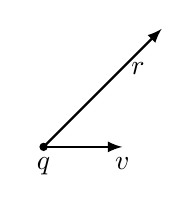
\begin{tikzpicture}
    \def\r{1cm}
    \coordinate (q) at (0,0);
    \coordinate (v) at (\r,0);
    \coordinate (r) at (1.5 * \r, 1.5 * \r);
    
    \draw[thick, -latex] (q) -- node[pos=0, below] {$q$} node[pos=1, below] {$\Vec{v}$}(v);
    \draw[thick, -latex] (q) -- node[pos=0.8, below] {$\Vec{r}$}(r);
    
    \fill[] (q) circle (1.5pt);
\end{tikzpicture}
\end{center}
\end{wrapfigure}
Для тока $I$ можно записать
\begin{equation*}
    I = \Vec{j} \cdot \Vec{dS} = q \cdot n \cdot v \cdot dS
\end{equation*}
Где $\Vec{j}$ -- плотность тока, $\Vec{dS}$ -- поперечное сечение проводника, $e, n, v$:  заряд, концентрация и скорость электронов. Тогда закон Био-Савара-Лапласа:
\setlength{\abovedisplayskip}{3pt}\setlength{\belowdisplayskip}{1.5pt}\begin{equation*}
    d\Vec{B} = \frac{\mu_0 e n v S [d \Vec{l} \times \Vec{r}]}{4 \pi r^3}, \quad
    d\Vec{B} = \frac{\mu_0 e \overbracket[1pt][1pt]{n S dl}^{dN} [\Vec{v} \times \Vec{r}]}{4 \pi r^3}
\end{equation*}
Отсюда, если принять $dN = 1$, поле одного заряда:
\begin{equation}
    \boxed{\Vec{B} = \frac{\mu_0 e}{4 \pi} \cdot \frac{[\Vec{v} \times \Vec{r}]}{r^3}}
    \label{eq:scmf}
\end{equation}
Вспомним формулу для величины напряженности электрического поля:
\begin{equation*}
    \Vec{E} = \frac{1}{4 \pi \varepsilon_0} \frac{q \Vec{r}}{r^3}
\end{equation*}
Заметим, что если загнать скаляры в векторное произведение $\displaystyle\Vec{B} = \left[\Vec{v} \times \frac{\mu_0 q \Vec{r}}{4 \pi r^3}\right]$
\begin{equation*}
    \Vec{B} = \mu_0 \varepsilon_0 [\Vec{v} \times \Vec{E}] \Longrightarrow \frac{1}{\sqrt{\mu_0 \varepsilon_0}} = c^2 \Longrightarrow \boxed{\Vec{B} = \frac{[\Vec{v} \times \Vec{E}]}{c^2}}
\end{equation*}
\setlength{\abovedisplayskip}{12.0pt plus 3.0pt
minus 7.0pt}
\setlength{\belowdisplayskip}{12.0pt plus 3.0pt
minus 7.0pt}

Отсюда связь магнитного и электрического поля. 